\documentclass[letterpaper, 10 pt, conference]{ieeeconf}

\IEEEoverridecommandlockouts
\overrideIEEEmargins              

\usepackage{cite}
\usepackage[pdftex]{graphicx}
\graphicspath{pictures/}
\DeclareGraphicsExtensions{.pdf,.jpeg,.png,.eps}
\usepackage{epstopdf}
\usepackage[cmex10]{amsmath}
\usepackage[caption=false,font=footnotesize]{subfig}
\usepackage{dblfloatfix}
\usepackage{fixltx2e}
\usepackage{color}
\usepackage{verbatim}
\usepackage{textcomp}
%\usepackage{algorithm2e}
%%\usepackage{algorithmicx}
%\makeatletter
%\newcommand{\removelatexerror}{\let\@latex@error\@gobble}
%\makeatother
%\hyphenation{op-tical net-works semi-conduc-tor}

% paper title
% can use linebreaks \\ within to get better formatting as desired
\title{\LARGE \bf
Applied Robotics for Installation and Base Operations \\for Industrial Hygiene}

%(ARIBO-IH)
% paresh comment: I will let you decide, but i think the title below is more descriptive but don't
% 					know if it will hurt your chances in TePra selection

% paresh suggested title:

% Autonomous Robotics for Installation and Base Operations Industrial Hygiene (ARIBO-IH) using an Unmanned Ground Vehicle (UGV) via Web-based User Interface for Command and Control

% author names and affiliations
% use a multiple column layout for up to three different
% affiliations
\author{Christopher Korpela, Kenneth Chaney, and Pareshkumar Brahmbhatt
\thanks{Manuscript received December 1, 2014. This work was supported in part by the Tank Automotive Research Development and Engineering Center (TARDEC). The views and conclusions contained herein are those of the authors and should not be interpreted as necessarily representing the official policies or endorsements, either expressed or implied, of the U.S. Government or TARDEC.}
\thanks{C. Korpela is with the United States Military Academy at West Point, NY 10996 USA \tt\small{christopher.korpela{@}usma.edu}}
\thanks{K. Chaney is with Drexel University in the Department of Computer Engineering \tt\small{kpc49{@}drexel.edu}}
\thanks{P. Brahmbhatt is with the University of Nevada, Las Vegas in the Department of Mechanical Engineering \tt\small{brahmbha{@}unlv.nevada.edu}}}


\begin{document}

\maketitle
\thispagestyle{empty}
\pagestyle{empty}

%%%%%%%%%%%%%%%%%%%%%%%%%%%%%%%%%%%%%%%
% Abstract
\begin{abstract}
A framework is proposed for Industrial Hygiene inspection using a remotely-operated ground vehicle with multiple sensor payloads attached to it for detecting various hazardous gases and chemicals. A control scheme and a graphical user interface between the vehicle and operator is strictly mandated for tasks requiring remote inspection. By leveraging existing navigation and path planning algorithms, the system can autonomously patrol hazardous areas and relay all measurements taken back to the user. This paper presents recent validation testing results of the system and its sensors using the proposed industrial hygiene framework.
\end{abstract}


%%%%%%%%%%%%%%%%%%%%%%%%%%%%%%%%%%%%%%%
% Introduction
\section{Introduction}\label{sec:introduction}

Throughout the Army, Industrial Hygiene (IH) teams are responsible for inspection, environmental reconnaissance, and emergency response. Industrial hygiene is an integral part of installation force protection and is an important component of an installation’s toxic industrial chemical spill planned response. Current best practices for conducting the IH mission requires direct human exposure to these hazardous environments. Robotic systems offer the potential to remove humans from these dangerous situations while maintaining the reliability and accuracy of the response team. Applying robotic solutions to this domain also contribute to the Department of Defense (DoD) unmanned systems goals outlined in the Unmanned Systems Integrated Roadmap FY2011-2036 \cite{roadmap}. Furthermore, robotic IH solutions are a force multiplier because these systems can be sent into a hazardous environment, parked, and allowed to collect data autonomously. Additionally, using robotic platforms for the IH environment is faster and safer than equipping and decontaminating a human. Finally, if successful, this project has potential DoD-wide application. 

\subsection{Trends}

Aging stocks of munitions and newly developed systems are creating larger quantities of dangerous materials that require monitoring and potentially, emergency response. In the current austere fiscal environment, enlarging a trained, professional IH team is a significant challenge. It is desirable to reuse/re-purpose existing inventory and to improve efficiency where possible.  One way to accomplish this goal is to automate tasks using technology such as robots and networked systems. This automation can allow a smaller team of trained personnel to effectively manage a large group of tasks.

\begin{figure}
	\centering
	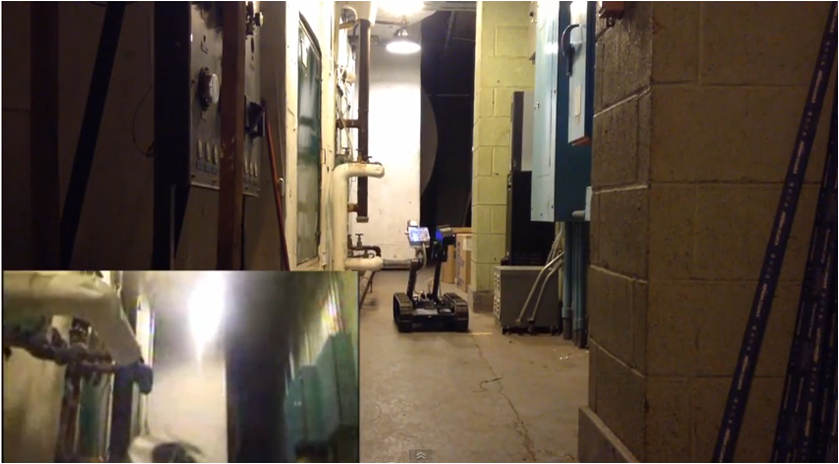
\includegraphics[width=0.48\textwidth]{./pictures/concept}
	\caption{ARIBO-IH prototype vehicle inspecting a gas leak in a notional hazardous site.}
	\label{fig:concept}
\end{figure}

\subsection{Problems}

An Industrial Hygiene mission is to reduce soldier and employee exposure to environmental factors and stresses including:  chemical (e.g., liquid, particulate dust, fumes, mist, vapor and gas), physical (e.g., electromagnetic radiation, temperature, ambient pressure, noise, vibration and ionizing radiation), and biological (e.g., agents of infectious diseases, insects, mites, molds, yeasts, fungi, bacteria and viruses) elements. The majority of hazards come from industrial processes on Army installations. Army industrial hygiene personnel are at risk from exposure to these hazardous environments in the conduct of their duties. Additionally, rapidly equipping human teams for response to incidents and post-action decontamination pose difficult challenges.  

\subsection{Benefits}

Through the use of robotic-enabled ground vehicles in a structured, controlled environment, the ARIBO-IH pilot will increase researchers’, manufacturers’, and users’ understanding and familiarity of these systems in real-world operational scenarios. The ARIBO-IH pilot safely provides the service of IH inspections, removing the human IH professional from a potentially hazardous situation while reducing cost. Additionally, the project will facilitate the design, standardization, deployment, and supervision of the resulting ARIBO-IH inspection robots. Finally, by using United States Military Academy (USMA) cadets as researchers, they are exposed to Army technologies and systems at the beginning of their careers.  The benefits of generating officers with technological backgrounds in robotics systems is paramount to achieving the DoD’s long term unmanned systems goals.

\subsection{Example Uses}
The robotic systems developed under this project could be employed in a number of situations to include:
\begin{itemize}
	\item Environmental reconnaissance in routine industrial hygiene tasks and emergency response
	\item Weather station at the emission source
	\item Ventilation duct inspection
	\item Investigate suspected terrorist devices
	\item Site abatement or mitigation projects
\end{itemize}

This paper presents a solution to the industrial hygiene problem using a small ground vehicle equipped with a sensor package. A control scheme for the system (Fig.~\ref{fig:concept} is implemented to allow for unattended operation in a known environment. Sec.~\ref{sec:model} details the kinematic and dynamic model for the system. The hardware and software components are found in Sec. \ref{sec:hardware}. Section~\ref{sec:results} presents validation results and sensor testing.

%%%%%%%%%%%%%%%%%%%%%%%%%%%%%%%%%%%%%%%
%Section: Hardware
\section{Mobility Platform}\label{sec:platform}

The iRobot PackBot is a fielded small robot used primarily for bomb disposal \cite{iRobot,Hogg2002}. The design is ``semi-modular'' where payloads can be installed to the base chassis, but they can only be installed in specific configurations, and when the software is properly configured. The integration of new payloads is often difficult and expensive. The vehicle uses military BB-2590 Li-Ion rechargeable batteries. While they have been widely deployed to both Iraq and Afghanistan, the PackBot is very expensive to purchase and maintain and overall reliability has been a challenge. There are two different generations: the obsolete 500 version and the current production 510 version. Many parts are interchangeable between the two models. The U.S. Army has discontinued the PackBot and no longer supports it as a program of record.

\begin{figure}
	\centering
	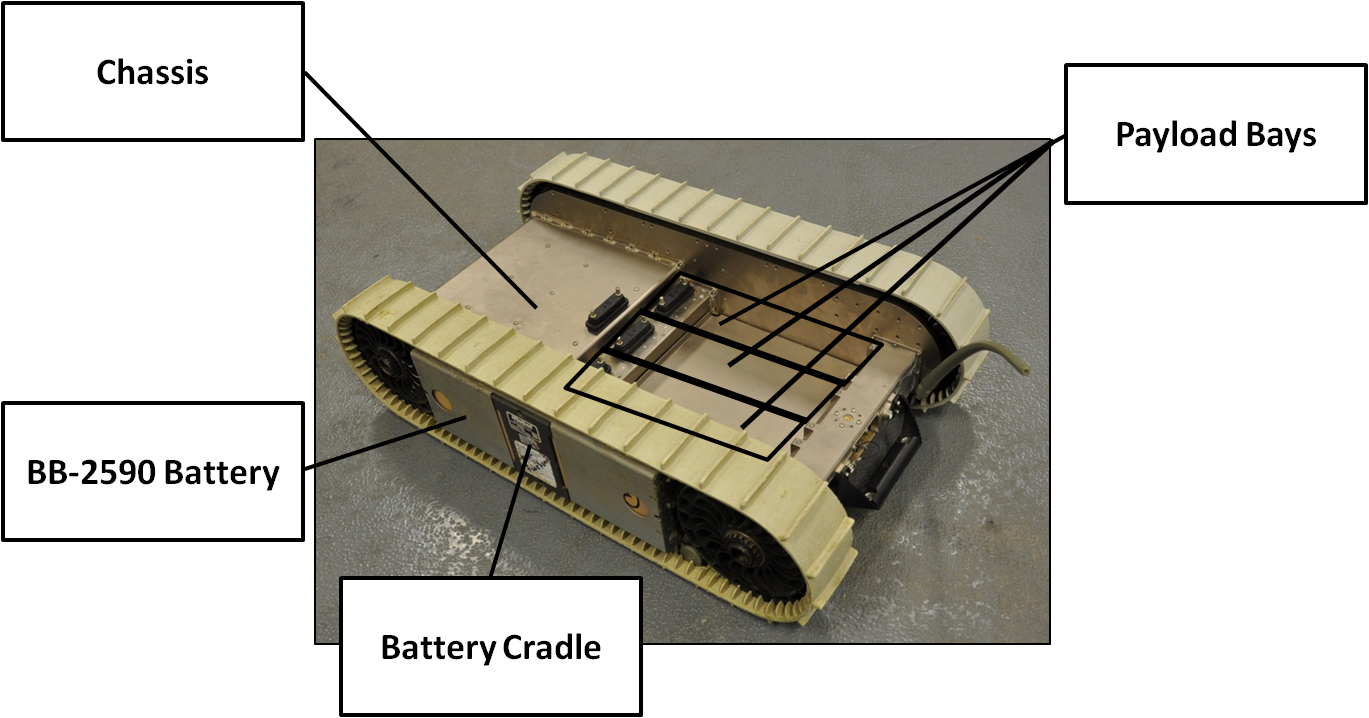
\includegraphics[width=0.48\textwidth]{./pictures/packbot1.png}
	\caption{Anatomy of the GVR-Bot.}
	\label{fig:packbot}
\end{figure}

With a large inventory of unused and unsupported robots, the RS-JPO (Robotic Systems Joint Program Office) funded a 12 month effort to implement IOP (Interoperability Profile V2, using JAUS which is the Joint Architecture for Unmanned Systems) on the existing PackBot platforms. Creating a kit design for retrofitting all fielded PackBots would reduce costs of maintaining the aged fleet. The standardized version of the PackBot makes for a good research platform due to a number of reasons:
\begin{itemize}
	\item Open architecture
	\item Design is completely government-owned
	\item Designed for IOP V1 compliance
	\item Cost is relatively low
\end{itemize}

The research platform became known as the GVR-Bot (Ground Vehicle Robotics is a branch of TARDEC) as shown in Fig.~\ref{fig:packbot}. The radio frequency was changed to 2.4 GHz so it could easily connect over standard and existing wireless Internet protocols. All of the internal electronics of the robot were replaced with new motherboards, interface boards, and motor controllers. Bootloaders were added to the internal control boards, thus allowing all of the software to be flashed without disassembling the robot. See Fig. \ref{fig:pcb} for an example printed circuit board configuration. The internal computer of the GVR-Bot manages linear and rotational accelerations/velocities of the vehicle, odometry, orientation, battery levels, GPS, and communications. The GVR-Bot used for IH missions contains an external embedded computer (Intel Core i7) to perform navigation and obstacle avoidance tasks, video monitoring, sensor integration through a mote (Libelium Waspmote), and collects LiDAR data using a Velodyne HDL-32E.   

\begin{figure}[b]
	\centering
	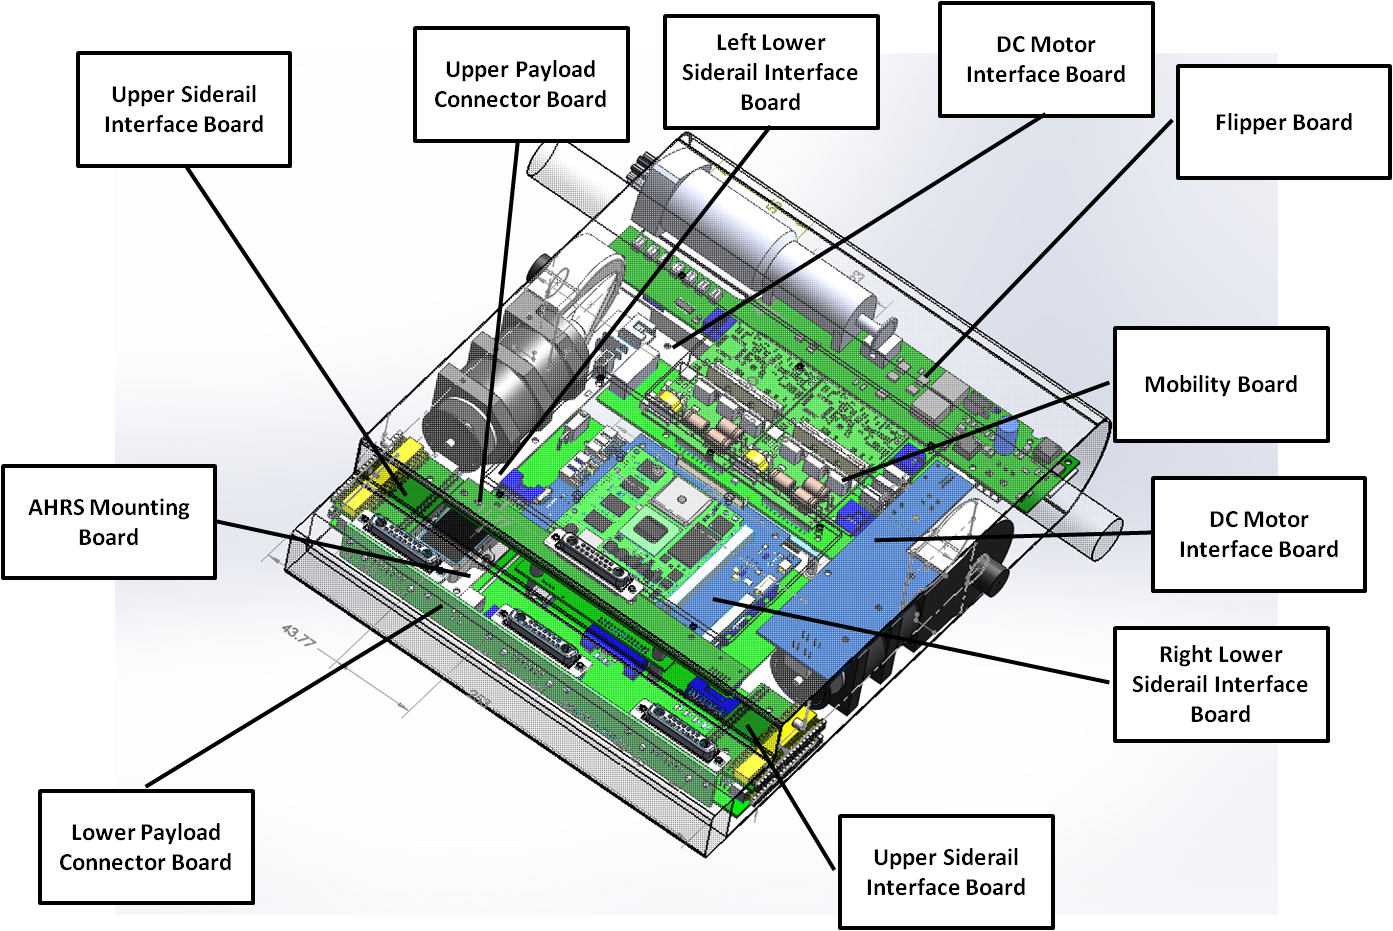
\includegraphics[width=0.48\textwidth]{./pictures/pcb.png}
	\caption{Front assembly interface board. This printed circuit board and sub-assemblies are part of the complete electrical component redesign of the Packbot.}
	\label{fig:pcb}
\end{figure}

%  Add in stuff about lidar and how it moves up and down (pitches on Y) or yaws 180deg on Z (sweeping back-forth) sitting on its side 
%what about the kind of processing power it has on-board to do this slam crap 


%%%%%%%%%%%%%%%%%%%%%%%%%%%%%%%%%%%%%%%
%Section: User Interface
\section{User Interface Software Suite}\label{sec:ui}

A standardized graphical user interface (GUI)\footnote{GUI is synonymous with Operator Control Unit (OCU).} was developed to be robust, intuitively usable by anyone, and serve as an all-in-one software suite (Fig. \ref{fig:gui_flow}) for servicing inputs and outputs via Robot Operating System (ROS) which acts as the backend of the GUI. The GUI frontend seen by the user is responsible for relaying environmental sensor and navigation data. The GUI software backend is standardized for use on any ground robot that is able to traverse through a 3 degree of freedom (DOF) work space ($x$,$y$,$\theta$) using an under-actuated controller. The user is able to control the robot's movement with a single virtual joystick controlling forward motion and turning. A wrapper is written to translate the joystick commands to actual motor commands. A second virtual joystick is available and dedicated to manipulating the camera viewpoint towards regions of interest in real time. This joystick allows the user to control a pan-tilt unit attached to the camera base. The camera feed and joystick bandwidth is automatically adjusted and delegated based on the bandwidth that is available at a particular instance between the robotic platform and the control unit. The GUI will alert the user if any bandwidth limits have been reached and will attempt to provide the user with the most up-to-date sensor and video data to allow the user to make the most informed decision possible in a given situation. Bandwidth concerns have a real impact upon mobile safety applications and must be taken into account; \cite{erikson2013} goes into further detail about how mobile constraints can alter the user interface and backend.

\begin{figure}
	\centering
	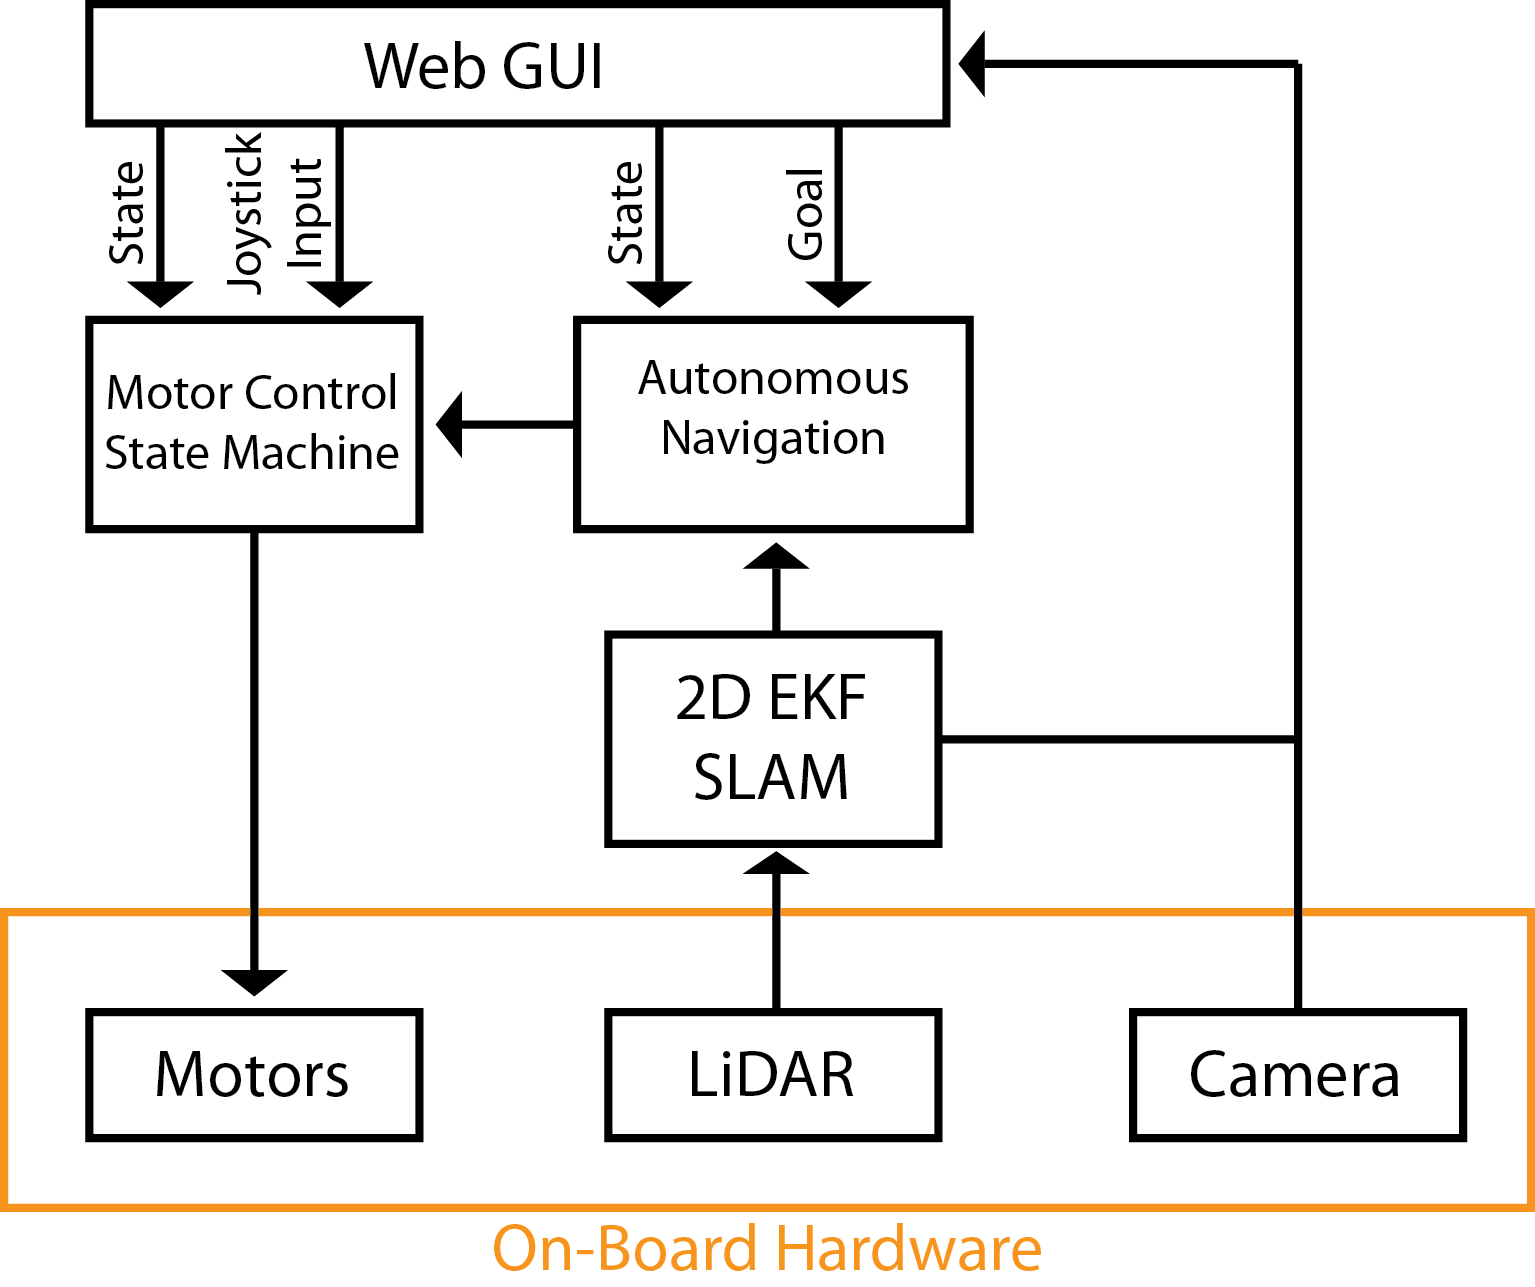
\includegraphics[width=0.48\textwidth]{pictures/Korpela_GUI.png}
	\caption{System flow of individual robot interface.}
	\label{fig:gui_flow}
\end{figure}

%To use this GUI for other ground robot platforms, all that would need to be developed is the wrapper code that translates the joystick into movement, assuming a different robot platform will have a different language coded onto its on-board system or motor controller. 

%While the control unit can be anywhere in the world, thus allowing the robot user to operate it through the internet or cloud service, there is better overall performance as well as lower latency in video stream, sensor data, and joystick data when the control unit is within the same compound as the robot. In ideal conditions, the user would be able to see and respond to any obstacle that is close by within low response time deltas, however under most conditions this isn't possible nor reasonable to expect. Low level obstacle avoidance function aids with basic navigation and reduces the probability of a crash that may be unforeseen by the user. The risk of the robot crashing into an obstacle cannot be completely mitigated because of several factors, but a few are real world delays in the data stream, loss of user's focus, lapses in data due to packet loss, the camera view is facing away from the obstacle, and connection loss.

%Another feature that has been built into the GUI is controlling based on way points instead of direct control over the robot. This allows for the user to click on the map to command the robot to navigate to the destination if possible. A 2D map is generated using SLAM from a LIDAR mounted on the robot--only differentials in the map are sent over the network. So while the initial connection may be slow, the delay during use is reasonalble. The 2D point that the user inputs is then fed into the navigation stack to attempt to reach the end goal. A third mode that the robot can be put into is pure autonomous navigation where the user can view what the robot is doing but won't have any control over the robot. The controller's multiple functionality allows for the user to pick the most appropriate mode of operation for a particular point in time, or to help the robot if it ever gets stuck. This is an important consideration when developing a GUI that is meant for long term industrial use, as all robots will eventually encounter something that they don't know how to deal with. 

\subsection{Navigation Modes}

As previously mentioned, the GUI allows the user to utilize two joysticks with one being for robot motion, and the other for camera pan-tilt motion; this two joystick scheme constitutes the first control mode. The GUI is designed to feature additional control modes. The control modes change the level of autonomy the robot exhibits during its mission. This feature, of course, requires for the different control modes to be hard-coded into the robot to ensure full functionality, both in terms of autonomous motion and safety of equipment in the facility being traversed. The change in control modes helps reduce the probability of mission failure or loss of robot if the control unit loses connection to the robot. The modes also change the level of involvement of the user in navigation duties, thus allowing the user to focus on higher level duties such as finding sources of contamination. This reduction of mental fatigue on the user helps increase missions success. All navigation modes utilize the GUI built-in features of map updating when differentials are found, obstacle proximity alerts, and environmental sensor warnings. 

% or thorough sterilization of the robot's local environment
%The second navigation mode provided through the GUI lets the user move the robot via way point navigation, which is done through a 2-Dimensional (2-D) interactive map of the compound that is provided to both robot and control unit prior to start of the mission. The robot is given way point locations to reach on the interactive map by the user during the start of its mission to alleviate future bandwidth needs that may arise as the mission progresses, and as bandwidth becomes restricted with increased distance from the control unit. These way points are generated by the interactive map feature after translating user input given via a mouse click-action on the 2-D map. If, for any reason, the robot is incapable of navigating to a way point it sends a warning message to the user indicating that autonomy has been reduced, and the robot has reverted back to control mode 1. The user can then use 2 joysticks to manually  maneuver the robot further into the compound or return it to the start point. After a predetermined amount of time, with no user input in control mode 1, the robot elevates autonomy and reverses course to return to the mission's start position using the way points taken to arrive at its current position. 

The second navigation mode allows for full autonomous exploration of the environment regardless of having any \emph{apriori} knowledge of the environment or not having a map. The robot uses LIDAR-based SLAM-EKF \cite{weingarten2005ekf, castellanos2007robocentric} to generate a map if none exists already. The map data is held in the on-board PC of the robot and can be transmitted on demand or streamed live. All navigation and obstacle avoidance actions are recorded on the full 3-D map, as metadata, that is generated as the robot progresses through the environment. Video data can also be toggled on if the user desires to visually inspect mission progress. By default, in order to reduce bandwidth saturation, map data is not transmitted to let mission critical sensor data take transmission priority.  A fail-safe feature sends a warning message to the user to indicate that the robot has reverted back to Mode 1 for manual navigation. This only occurs if the robot is unable to continue through the environment or has encountered a navigational error in its on-board programming. If the user takes no action or the connection has been lost, the robot again elevates autonomy to its original setting to reverse course and return to the mission start position. 

\subsection{HTML Interface}

The desire to create a web-based control application has been explored since the inception of the Internet \cite{goldberg2002beyond}. The GUI is a web application that has all the mentioned features to be toggled on or off through a settings window which is separate from the main robot interaction window in order to reduce the clutter the user sees while performing a mission (Fig. \ref{fig:gui_screenshot}). This will reduce the likelihood that the user will mistakenly click or press the wrong button during mission critical moments. The aforementioned navigation modes can be toggled on-the-fly by the user and are accessible directly from the main robot interaction window. The GUI frontend itself is based on Robot Web Tools \cite{webtools,lee2012web} which is a set of modules that help create web-based robot control applications. It allows ROS software package messages and topics to be accessible through a web interface that is constructed using HTML5 and Javascript via a wrapper called \textit{rosjs} \cite{osentoski2011robots}. The GUI is essentially a web accessible overlay that allows the user to send and receive data across a connection between a ROS server, the control unit, and its corresponding ROS client, the robot. The advantage of using HTML5 is its cross-platform compatibility allowing the web application to be used by PCs, tablets, and smart phones \cite{hilton2014lightweight}. On the ROS client, the robot computer runs a \textit{roscore} node that uses a package called \textit{rosbridge} which allows socket-based access to ROS through Javascript \cite{crick2011rosbridge}.

\begin{figure}
	\centering
	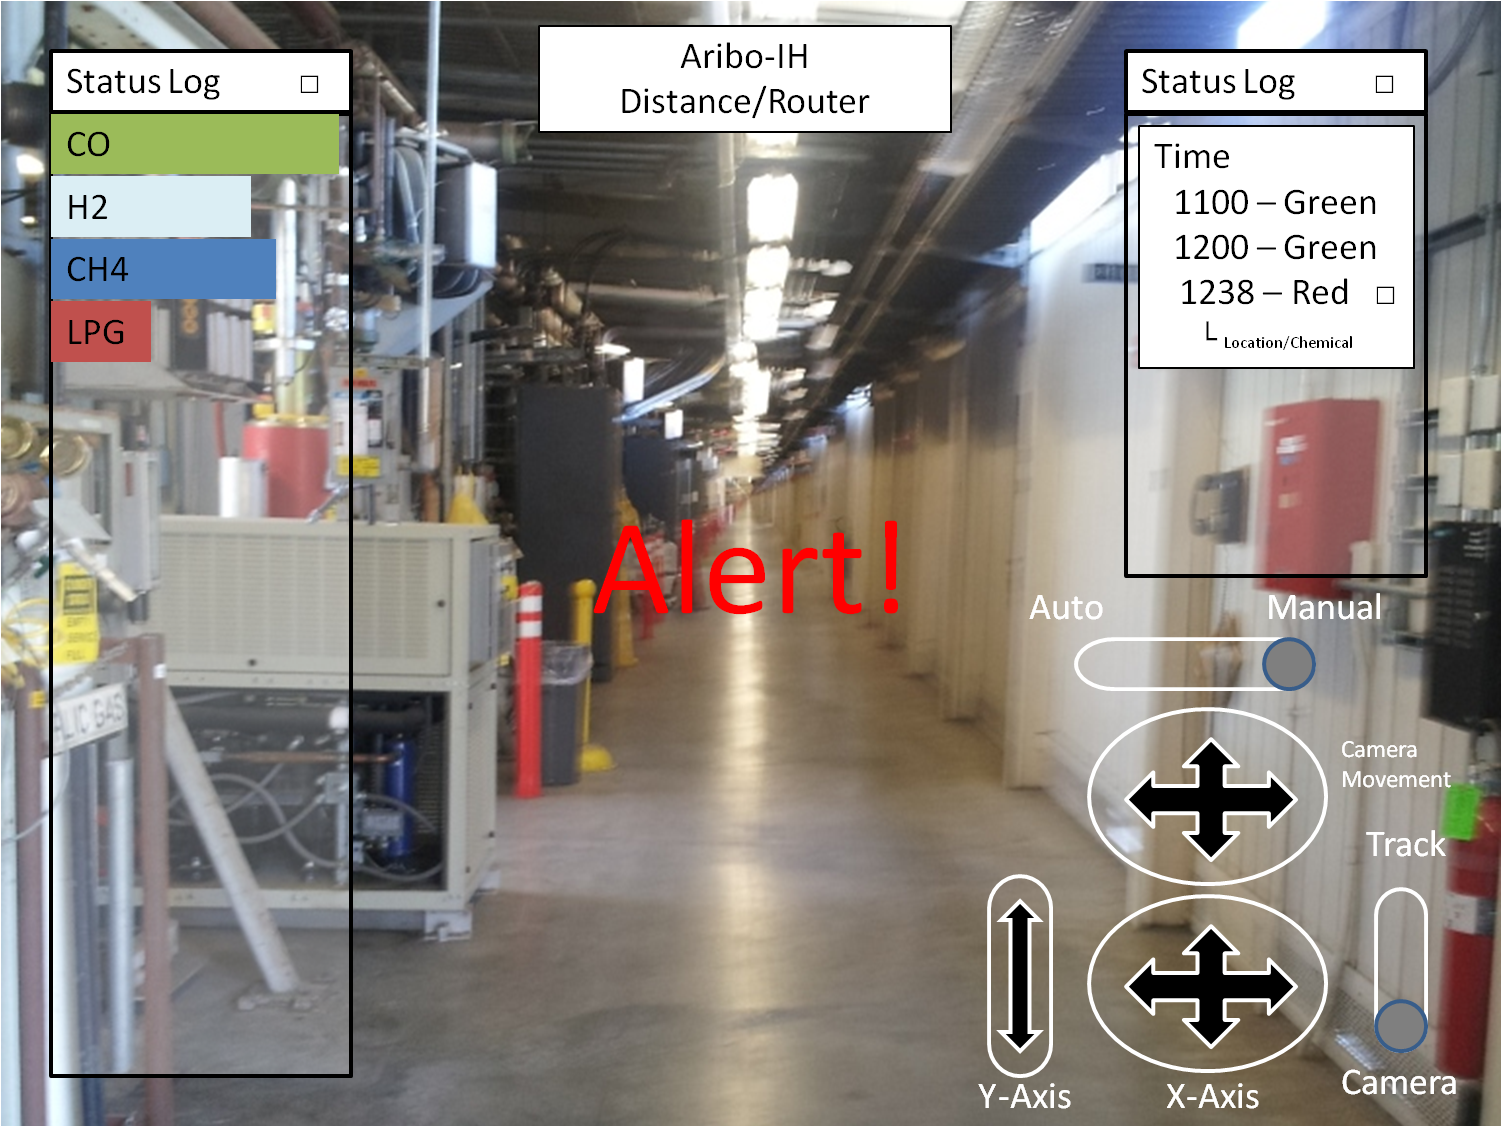
\includegraphics[width=0.48\textwidth]{pictures/gui-slac.png}
	\caption{Screenshot of the developed web-based GUI allowing for view of the camera and 2-D map.}
	\label{fig:gui_screenshot}
\end{figure}


%%%%%%%%%%%%%%%%%%%%%%%%%%%%%%%%%%%%%%%
%Section: Sensors
\section{Sensors}\label{sec:sensors}

The sensor sub-system links directly to the user interface by providing plug-and-play functionality depending on mission requirements. Using modular sensors with standard interfaces and protocols, a wide variety of sensors can be fitted on the GVR-Bot. Power is provided through the vehicle's two BA-2590 batteries for up to 2 hours as the batteries each have 14 Ah, and with the full system operating, the current drain does not exceed 3A. The power system used for the prototype can support more powerful sensors if required. The initial prototype can detect gases, liquids, and atmospheric conditions as shown in Fig.~\ref{fig:params}.

\begin{figure}[b]
	\centering
	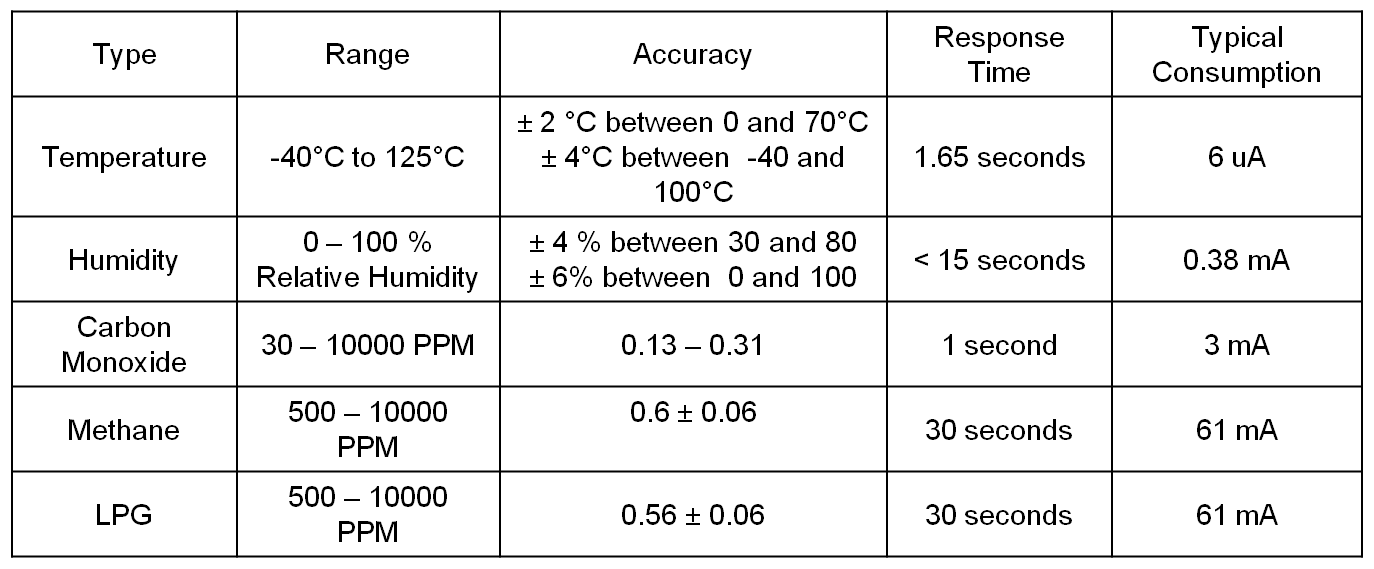
\includegraphics[width=0.48\textwidth]{./pictures/sensor_params.png}
	\caption{Types of sensors showing accuracy, response time, and power consumption rates.}
	\label{fig:params}
\end{figure}

For data acquisition, a microcontroller is used to process the sensor data and generate the data packets that are sent through the robot's embedded computer and wirelessly transmitted to the GUI to be stored in a database and displayed for the user. The software makes it possible for a user to modify, add, or subtract the current sensors used in order to fit the desired application. Furthermore, the multiple I/O channels on the microcontroller allow for easy access to integrate additional sensors. The structure of the sensor packet is scalable to add additional information as shown in Table \ref{tab:packet}. The received data is saved in a database to provide a history of the event readings. As explained in the user interface section, the familiarity of the GUI ensures that the user does not have to learn a completely new control interface. A sensor toolbar was developed to mesh with the robot's current user interface to provide live data readings. When a sensor reading passes a dangerous threshold, the toolbar will change colors to alert the operator. Under each sensor, a button displays a graph of the sensor's history.

\begin{table}
	\centering
	\begin{tabular}{ |l|l|l| }
		\hline
		\multicolumn{3}{ |c| }{Sensor Packet} \\
		\hline
		Sensor ID & Binary & 1 byte \\ \hline
		Data Type & Binary & 1 byte \\ \hline
		Data Length & Binary & 1 byte \\ \hline
		Data & (data type) & (data length) bytes \\
		\hline
	\end{tabular} 
	\caption{Sensor packet structure used to communicate sensor data back to the user interface.}
	\label{tab:packet}
\end{table}

%%%%%%%%%%%%%%%%%%%%%%%%%%%%%%%%%%%%%%%
%Section: Navigation
\section{Navigation}\label{sec:navigation}

The internal computer of the GVR-Bot passes sensor data to the on-board, external embedded computer for processing, map generation, and development of a navigation scheme. The external embedded computer is directly connected and receives updates from the LIDAR in real-time. The tilting capability of the LIDAR allows 3-D point cloud data to be collected for use in developing a 3-D navigation solution. For ARIBO-IH missions, accurate inertial measurements are not required because navigation occurs in highly structured indoor environments, and odometry data helps mitigate errors in position. The computer then uses the laser data to generate a 2-D planar occupancy grid map. The technique of using occupancy grid maps based on LIDAR scans is being implemented because it can be done at a low cost computationally, and it is a proven approach for localizing a ground robot in a real-world setting \cite{thrun2005probabilistic,kohlbrecher2011flexible}. The 2-D SLAM information is coupled with a 3-D pose estimate that is generated using an Extended Kalman Filter (EKF). This coupling allows the 2-D planar map to be overlayed with robot pose data estimated via EKF. 

This information is locally stored in memory for purposes of future unplanned events that may occur during the mission, such as connection loss. The highly detailed 3-D map and a 2-D planar map are generated, while a coarser version of the 2-D map is created for the purposes of wireless transmission to the control unit to be displayed on the GUI for the user. This multi-resolution map representation does not rely on any type of filtering or downsampling, but it simultaneously generates multiple maps of different resolutions that have scalability and low cost computationally. This approach is further described in \cite{kohlbrecher2011flexible,habbecke2006iterative}. The high computation capability of the computer allows for both the SLAM and 3-D EKF components to be run at soft real-time with a low enough latency in calculation that it is negligible compared to actual or hard real-time 3-D navigation schemes.

\subsection{Practical Implementation}\label{sec:practical}

The Stanford Linear Accelerator Center (SLAC) National Accelerator Laboratory has partnered with TARDEC and West Point to field a GVR-Bot for use in the two-mile long tunnel. Currently, maintenance crews must traverse the tunnel and visually inspect for gases, liquids, radiation, vibrations, ultrasonic frequencies, and atmospheric effects that could be harmful to humans. As previously described, the GVR-Bot navigates the tunnel as shown in Fig.~\ref{fig:tunnel} which is generally clear of debris and has known features throughout the corridor. Sensor packages are installed as described in Sec. \ref{sec:sensors} and the graphical interface provides robot pose and environmental information as discussed in Sec. \ref{sec:ui}.

\begin{figure}
	\centering
	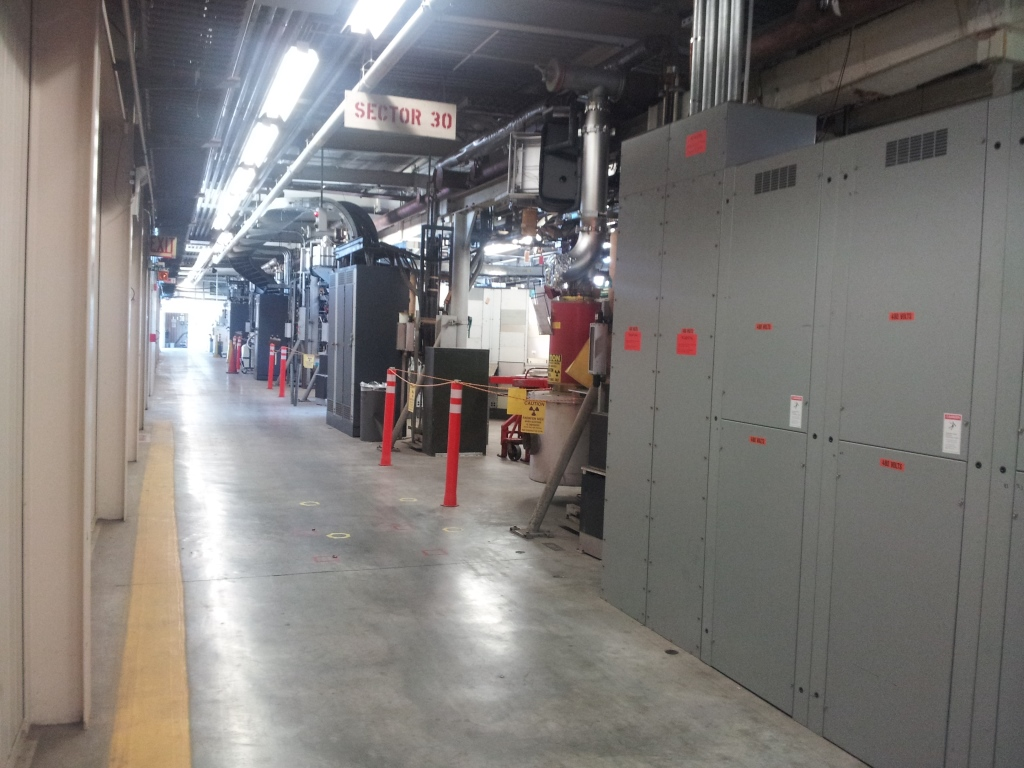
\includegraphics[width=0.48\textwidth]{./pictures/slac-tunnel.jpg}
	\caption{Interior corridor of SLAC tunnel.}
	\label{fig:tunnel}
\end{figure}


%%%%%%%%%%%%%%%%%%%%%%%%%%%%%%%%%%%%%%%
%Section: Results
\section{Sensor Testing and Results}\label{sec:results}

Since gas sensors are inherently inaccurate due to their manufacturing processes and biases, each sensor had to be calibrated by graphing the output of each sensor compared to the known gas in the testing environment. The testing environments consists of 1.0 liter sealed containers with the sensor inserted into one end and a septum for needles inserted in the other as illustrated in Fig. \ref{fig:sensor}. The 1.0 liter volume simplified the calculations in parts-per-million (ppm) and each gas was introduced to the environment via a syringe and needle.

\begin{figure}
	\centering
	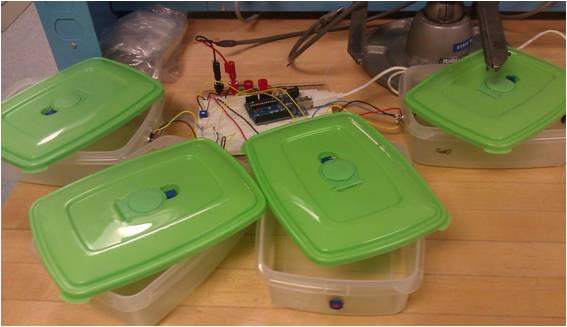
\includegraphics[width=0.48\textwidth]{./pictures/sensor.jpg}
	\caption{Testing environments (from left to right): MQ-4, MQ-6, MQ-7, and MQ-8 sensors.}
	\label{fig:sensor}
\end{figure}

By comparing the sensor output (x-axis) to the known concentration of gas in the testing environment (y-axis), a curve is formed, which can be best fit to an exponential curve by focusing the comparison on moderately to severely dangerous gas concentrations, which is approximately 2,000 to 10,000 ppm. The best fit equation for the most accurate test is used in software to correct the sensor output to the most accurate output for transmission to the operator through the GUI. Figs. \ref{fig:methanetoxic}-\ref{fig:hydrogen} display the graph for the MQ-4 (Methane) sensor along with the graphs for MQ-6 (Liquefied Petroleum Gas), MQ-7 (Carbon Monoxide), and MQ-8 (Hydrogen) sensors.

\begin{table}
	\centering
	\begin{tabular}{|c||c|}
		\hline
		Test & \(R^2\) \\ \hline \hline
		Methane Toxicity & 0.996 \\ \hline
		Methane Test & 0.994 \\ \hline
		LPG Test & 0.999 \\ \hline
		CO Test & 0.998 \\ \hline
		Hydrogen Test & 0.969 \\ \hline
	\end{tabular}
	\caption{\(R^2\) values associated with fit curves in Figs. \ref{fig:methanetoxic}-\ref{fig:hydrogen}}
\end{table}

\begin{figure}
	\centering
	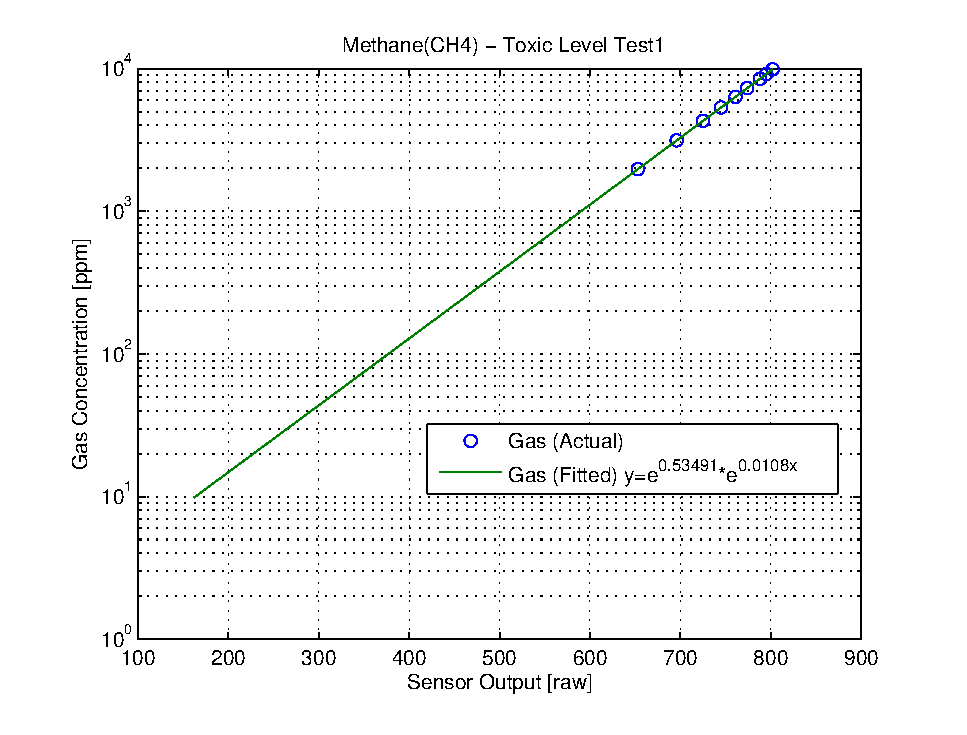
\includegraphics[width=0.4\textwidth]{./matlab/MethaneToxic.eps}
	\caption{Methane toxic levels. Threshold values are used to determine levels that are hazardous to humans.}
	\label{fig:methanetoxic}
\end{figure}

\begin{figure}
	\centering
	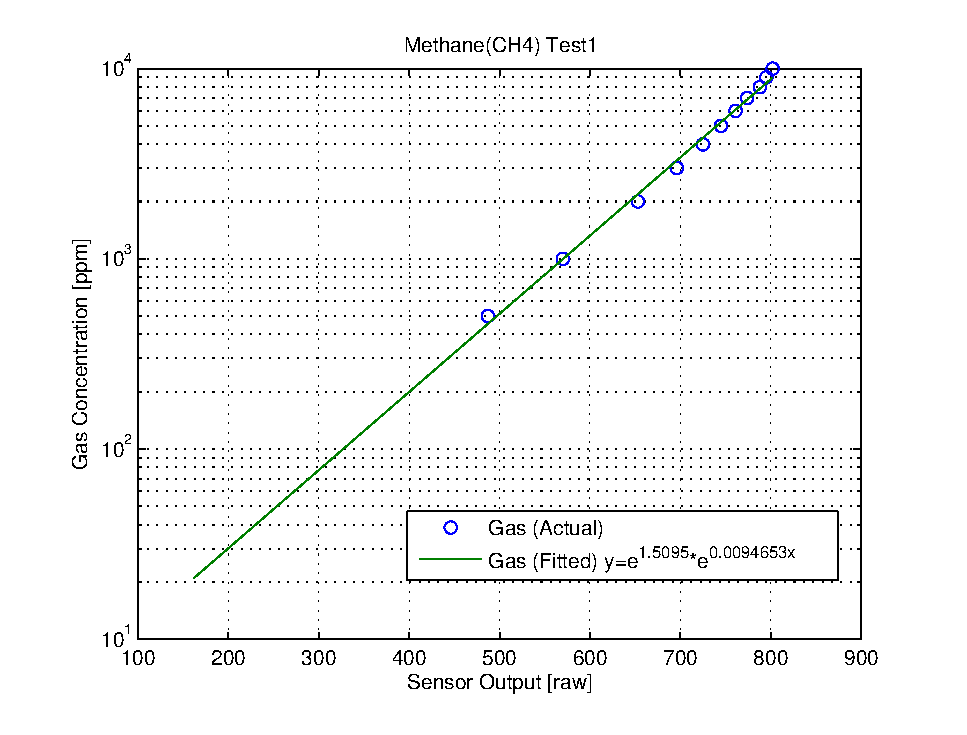
\includegraphics[width=0.4\textwidth]{./matlab/MethaneTest1.eps}
	\caption{Methane Gas test.}
	\label{fig:methanetest}
\end{figure}

\begin{figure}
	\centering
	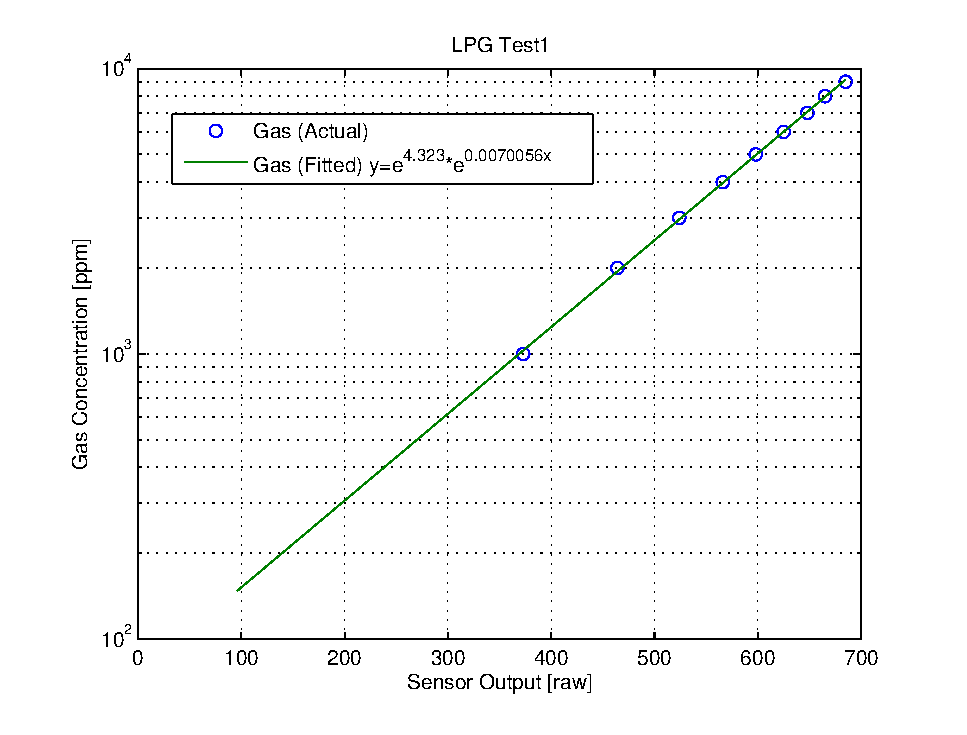
\includegraphics[width=0.4\textwidth]{./matlab/LPG.eps}
	\caption{Liquefied Petroleum Gas test.}
	\label{fig:lpg}
\end{figure}

\begin{figure}
	\centering
	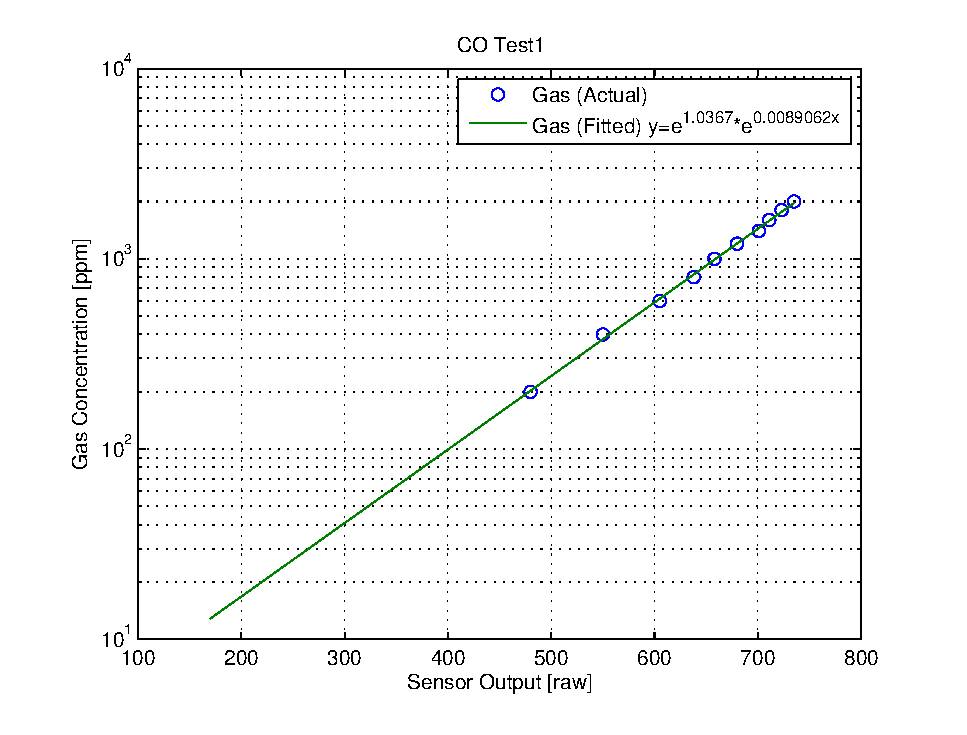
\includegraphics[width=0.4\textwidth]{./matlab/COTest1.eps}
	\caption{Carbon Monoxide test.}
	\label{fig:co}
\end{figure}

\begin{figure}
	\centering
	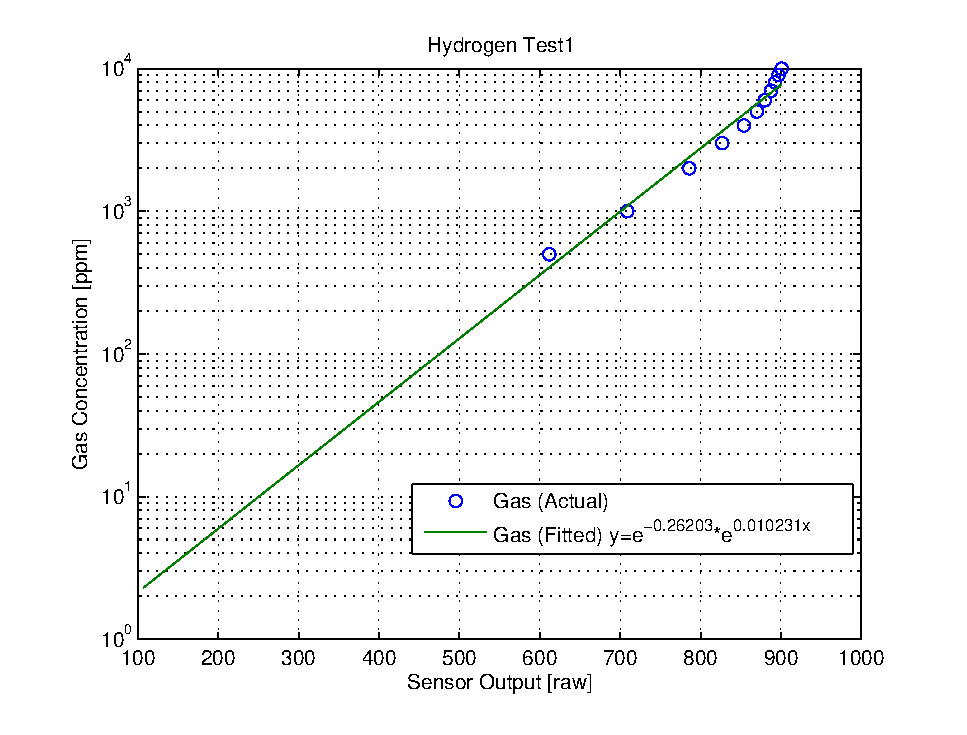
\includegraphics[width=0.4\textwidth]{./matlab/HydrogenTest1.eps}
	\caption{Hydrogen test.}
	\label{fig:hydrogen}
\end{figure}

Using the correction equations in software with the given sensor outputs, the final results closely match the expected concentrations. The corrected outputs will be able to discern the difference between a safe and a dangerous environment. 


%%%%%%%%%%%%%%%%%%%%%%%%%%%%%%%%%%%%%%%
% Conclusions
\section{Conclusions}\label{conclusions}
Industrial Hygiene monitoring and response functions possess the potential for improving efficiency and safety through the use of robots. Robotic systems such as the GVR-bot can remove humans from dangerous environments while accurately and reliably conducting tasks that are critical to operations on all Army installations. These improvements in efficiency and safety can be obtained in a fiscally responsible manner through the use of existing Army systems. Additionally, research conducted at the Academy benefits the Army long-term by exposing future officers to Army programs and technology at the beginning of their career.

%%%%%%%%%%%%%%%%%%%%%%%%%%%%%%%%%%%%%%%
% Acknowledgments
\section{Acknowledgments}\label{acknowledgments}
The authors would like thank Edward Straub, David Tenenbaum, and Ty Valascho from TARDEC among others for their support, guidance, and expertise on this project. We would also like to acknowledge the students for ARIBO-IH: Francis Abbey, Marques Avery, Matthew Campbell, Andrew Frakes and Ji Kim.

%%%%%%%%%%%%%%%%%%%%%%%%%%%%%%%%%%%%%%%

%\addtolength{\textheight}{0cm}  % This command serves to balance the column lengths
                                  % on the last page of the document manually. It shortens
                                  % the textheight of the last page by a suitable amount.
                                  % This command does not take effect until the next page
                                  % so it should come on the page before the last. Make
                                  % sure that you do not shorten the textheight too much.

%%%%%%%%%%%%%%%%%%%%%%%%%%%%%%%%%%%%%%%

\bibliographystyle{bibliography/IEEEtran}
\bibliography{bibliography/IEEEabrv,bibliography/bibliography}

\end{document}
